% @file   thesis.tex
% @brief  graduation thesis of Shibaura Institute of Technology
% @author Kataoka Nagi al18036[at]shibaura-it.ac.jp
% @date   2021-12-21 15:19:48
% $Version:   1.0
% @parHistory
% add
% Copyright (c) 2021 Kataoka Nagi

\documentclass[12pt,a4j]{jreport}
\setcounter{secnumdepth}{5}
\usepackage[dvipdfmx]{graphicx}
\usepackage{amsmath,amssymb}
\usepackage{comment}
\usepackage{graphicx}
\usepackage{here}
\usepackage{bm}
\usepackage{url}
\usepackage{otf}

\renewcommand{\baselinestretch}{1.5}

\renewcommand{\bibname}{参考文献}





\begin{document}


%%%%%%%%%%%%%%%%%%%%%%%%%%%%%%%%%%%%%
% 表紙
%%%%%%%%%%%%%%%%%%%%%%%%%%%%%%%%%%%%%
\begin{titlepage}

\begin{center}

\vspace*{2cm}
\Large 2021 年度 芝浦工業大学 工学部 情報工学科\\

\vspace*{1.0cm}
\Huge 卒 \qquad 業 \qquad 論 \qquad 文\\
\vspace*{2.5cm}

\Large 主張と根拠のクラスタを用いた\\多様な主張を提示するニュース推薦手法の提案

\vspace{4cm}
\begin{tabular}{ll}
\vspace*{2mm}
学籍番号 & \qquad $\mathbf{AL18036}$ \\
\vspace*{2mm}
氏\phantom{  }名 & \qquad 片岡 \quad 凪   \\
\vspace*{2mm}
指導教員   & \qquad 木村 \quad 昌臣
\end{tabular}
\end{center}
\end{titlepage}



% \begin{abstract}
% このファイルは,情報工学科卒業論文の推奨テンプレートである.概要書とは異なり,卒業論文本体のテンプレートはあくまで推奨であるので,このテンプレートを下にして文字サイズや行間などを修正したものを利用しても良く,またこのテンプレートを使わなくても良い.

% この部分の研究概要では,研究背景,解決したい問題,研究目的,提案手法,評価方法,評価の結果について簡潔に書く.
% 概要の有無は任意.
% \end{abstract}


{\makeatletter
\let\ps@jpl@in\ps@empty
\makeatother
\pagestyle{empty}
\tableofcontents
\clearpage}

\setcounter{page}{1} 
\pagestyle{plain}

%%%%%%%%%%%%%%%%%%%%%%%%%%%%%%%%%%%%%%%%%%%%%%%%%%%%%%%%%%%%
% 書式 
%%%%%%%%%%%%%%%%%%%%%%%%%%%%%%%%%%%%%%%%%%%%%%%%%%%%%%%%%%%%
% 図の参照『図\ref{fig_nn}に3層のニューラルネットワークを示す』
% \begin{figure}[H]
% 	\centering
% 	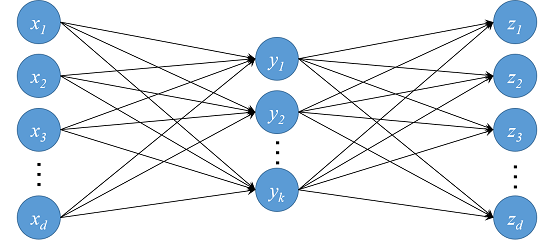
\includegraphics[keepaspectratio, width=120mm]{img/sample.png}
% 	\caption{提案法に用いた3層のニューラルネットワーク.キャプションにはこの図の説明を書く.}
% 	\label{fig_nn}
% \end{figure}

% 表の参照『表\ref{table_a}に手法Aおよび手法Bの正答率を示す』
% \begin{table}[H]
%   \caption{手法Aおよび手法Bの正解率と平均計算時間.}
%   \label{table_a}
%   \centering
%   \begin{tabular}{lcr}
% \hline
% 手法   & 正解率[\%]  &  計算時間[ms]  \\
% \hline \hline
% 手法A  & 92.3  & 512 \\
% 手法B  & 87.4  & 32  \\
% \hline
%   \end{tabular}
% \end{table}

% 参考文献『井尻らは,X線CTとデジタルカメラを用いた3次元モデリング法を提案した\cite{Ijiri18}.』
% 参考文献リスト『著者1, 著者2,...,著者N. タイトル. 論文誌or学会名, 巻, 号, ページ, 発表年. 』
% Webページ『著者. ページタイトル. ページURL(2021年7月31日参照).』


%%%%%%%%%%%%%%%%%%%%%%%%%%%%%%%%%%%%%%%%%%%%%%%%%%%%%%%%%%%%
\chapter{序論}
%%%%%%%%%%%%%%%%%%%%%%%%%%%%%%%%%%%%%%%%%%%%%%%%%%%%%%%%%%%%

(用紙や文字のなどのサイズには井尻先生のTeXテンプレートをそのまま利用しています)

(画像のサイズや\textbackslash newpageのタイミングは最後に調整します)

%%%%%%%%%%%%%%%%%%%%%%%%%%%%%%
\section{研究背景}
~
% @see 

%%%%%%%%%%%%%%%%%%%%%%%%%%%%%%
\section{研究目的}
~
% @see 

%%%%%%%%%%%%%%%%%%%%%%%%%%%%%%
\section{本論文の構成}
~
% @see 

%%%%%%%%%%%%%%%%%%%%%%%%%%%%%%%%%%%%%%%%%%%%%%%%%%%%%%%%%%%%
\chapter{本研究で用いる知識と技術}
%%%%%%%%%%%%%%%%%%%%%%%%%%%%%%%%%%%%%%%%%%%%%%%%%%%%%%%%%%%%

%%%%%%%%%%%%%%%%%%%%%%%%%%%%%%
\section{ニュース推薦システム}
多くのWebニュースサイトでは,様々なアルゴリズムを用いて読者の趣向に合わせた記事が提示されている.
アルゴリズムの例として,
読者が閲覧した記事に似た記事を推薦するコンテンツベースフィルタリング(Content-Based Filtering)や
似た趣向を持つ他の読者の閲覧記事を推薦する協調フィルタリング(Collaborative Filtering),
この2つや他のルールを併用したハイブリッドな手法などがある\cite{karimi_news_2018}.
このような読者にパーソナライズした推薦アルゴリズムをニュース推薦システム(News Recommender Systems)という.
アルゴリズムの評価指標には,記事の閲覧回数,閲覧記事のカテゴリ,読者の位置情報,他サイトの閲覧履歴や購買情報などがある.
% @see News recommender systems – Survey and roads ahead

%%%%%%%%%%%%%%%%%%%%%%%%%%%%%%
\subsection{ニュース推薦システムが生むバイアス}
\label{biases_generated_by_nrs}
パーソナライズするニュース推薦システムは,読者が得る情報に偏りを生む.
本節\ref{biases_generated_by_nrs}では,代表的な問題としてフィルターバブル問題とエコーチェンバー問題について記す.
本研究は,両問題の部分的な緩和を目指すものである.
% @see 0517-


\subsubsection{フィルターバブル問題}
Eli Pariserは2011年に,インターネットコンテンツの推薦アルゴリズムにパーソナライズ機能を組み込むことで生じる諸問題をフィルターバブル問題として提唱した\cite{pariser_beware_nodate}\cite{bruns_filter_2019}.
Pariserは,インターネット上で個人の趣向に合わせた限定されたコンテンツばかりが推薦されている状況を,ユーザーが泡の中に閉じ込められたような状態であると例えた.
例として,Facebookでユーザーが支持する政党ばかりが推薦され,Google検索でユーザーの居住地域と関係が薄い時事問題が推薦されるような状況が問題視されている.
泡の中の偏った情報は,新しいアイディアや異なる視点を生みにくくする.
市民が偏った情報ばかりに触れることで,民主主義が機能しなくなる可能性もある.

この泡の中で多様性のある情報を求めることは難しい.
なぜなら,泡の中の情報は個人のキャリアや行動履歴によって決まるため,個人で推薦アルゴリズムをコントロールできないことが多いからである.
同じ理由で,個人が泡の外の情報を特定できないことも大きな問題である.

% (to 提案手法)フィルターバブル問題を緩和する策として,推薦アルゴリズムの公開,個人が推薦アルゴリズムを管理できるオプションの作成,UIの工夫によるバブルの可視化がある.一方で,個人が推薦アルゴリズムを微調節したところで完全に情報の泡から脱することはできないとの指摘もある.UIでバブル内外を可視化しきるのは不可能 情報が多い 手軽

% @see 
% [1]E. Pariser, Beware online 「filter bubbles」, (1304298000). 参照: 1月 06, 2022. [Online Video]. Available at: https://www.ted.com/talks/eli_pariser_beware_online_filter_bubbles
% - きっかけ
%     - Facebook
%         - リベラル派だが進んで保守派と交流する
%         - ある日保守派の人たちが消えた
%         - どのリンクをクリックしているかFacebookがチェック
% - その他の例
%     - Google
%         - 57個のシグナルをチェック
%             - どんなPCを使っているか
%             - どのブラウザを使っているか
%             - 現在地は何処か
%         - 検索結果を調節
%         - 認識しにくい
%             - 自分の検索結果がどれほど他人のものと違うか分からない 
%         - 友人2人がGoogleで「エジプト」と検索
%             - エジプトのデモ関連記事が全くない
%                 - この頃大きな話題だったのに
%             - 他方はそればかり
%     - Yahoo!ニュース,Huffington Post,Washington Post,New York Times
%         - 様々な形でカスタマイズ
% - インターネットは私たちが見たいものを予測して見せている
%     - それは必ずしも見る必要があるものでない
%     - エリック・シュミット「全く何のカスタマイズもされていないものを 人々が見たり利用したりするのは とても難しくなるでしょう」
% - フィルターやアルゴリズムの結果
%     - フィルターに囲まれた世界
%         - あなた個人独特の情報世界となる
%         - 自分の世界に何が含まれるかは自分がどんな人で何をしているかによって決まる
%         - 何が取り入れられるかは自分次第でないのが問題
%             - Netflixのデータアナリスト「「アイアンマン」はすぐ届くのに 「スーパーマン」は 待ち時間が長い」
%                 - 利用者の計画的な向上心と衝動的な今の欲望が大きく対立
%                     - 「羅生門」を観たことがある人になりたい
%                         - 一方で4回目の 「エース・ベンチュラ」を観たい
%                     - 最良の編集は両面を見せる
%                     - フィルターは利用者が何を最初にクリックしたかを主に参考
%                         - そのようなバランスを崩す
%         - **何が削除されるか自分には見えない**
% - 放送社会の創設神話
%     - 編集者が情報の流れをコントロール
%     - インターネットが現れ編集者を追い払った
%     - 私たちは 繋がり合えるようになった
%         - 実際にはそうなっていない
%         - 人間の門番からアルゴリズムの門番にバトンが渡されている
%         - **アルゴリズムは編集者が持ち合わせていた倫理観念をまだ持っていない**
%             - アルゴリズムが関連性以外の要素も必要
%                 - 私たちが何を見て何を見ないか決めるのなら.
%             - 見たくないものや難しいもの,重要なものなども提示
% - 1915年
%     - 新聞は市民としての義務は考慮しない
%     - 市民が適切な情報を得ていないと民主主義は機能しない
%     - 情報のフィルターを行う新聞は重要
%         - ジャーナリズムの倫理が誕生
%     - ウェブ上で同じ問題に直面
%     - プログラムにこの責任を組み込みたい
%         - アルゴリズムを明白に
%         - 何が入ってくるか
%         - フィルターのルール
%         - 自分で何が削除されて何がされないか決められるように管理できるオプション
%         - 新しいアイデアや人々,異なる視点を提示すべき
%         - ウェブ上で私たちが孤立しないように
% [1]和俊笹原, 「ウェブの功罪」, 情報の科学と技術, vol. 70, no. 6, pp. 309–314, 2020, doi: 10.18919/jkg.70.6_309.
% - パーソナライゼーション
% - 選択の条件を知り得ない
% - ブラックボックスであることも
% - **アルゴリズムで虚偽情報が組み込まれることも**
% [1]亜斗夢園田, 寛人中島と不二夫鳥海, 「人気度に着目したニュース閲覧行動の変容分析」, 人工知能学会全国大会論文集, vol. JSAI2020, p. 1L5GS501-1L5GS501, 2020, doi: 10.11517/pjsai.JSAI2020.0_1L5GS501.
% - 自らが好む情報やそれを支持するコミュニティばかり接触することで,偏った考えがより強化される現象
% [1]敏弘神嶌, 昭太郎赤穂, 英樹麻生と淳佐久間, 「情報中立推薦システム」, 人工知能学会全国大会論文集, vol. JSAI2012, p. 3E1R61-3E1R61, 2012, doi: 10.11517/pjsai.JSAI2012.0_3E1R61.
% - フィルターバブル
%     - 利用者が接する情報の範囲に関する問題
%     - 推薦などの個人化技術により,利用者は,知らないうちに,自身が関心があるとされる限定された話題の情報のみにしか接しないようになっており,まるで『泡』の中に閉じ込めらたような状態
%     - 利用者がより新たな話題に関心をもつ機会が奪われたり,社会の中での情報や認識の共有が困難に
%     - フィルターバブル
%     - 推薦を含めた個人化技術によって
%     - 利用者が接する情報の話題の範囲が狭められたり,偏ったりすることが
%     - 利用者が知らないうちに行われるという問題
% [[1]E. BozdagとJ. van den Hoven, 「Breaking the filter bubble: democracy and design」, Ethics Inf Technol, vol. 17, no. 4, pp. 249–265, 12月 2015, doi: 10.1007/s10676-015-9380-y.](https://link.springer.com/article/10.1007/s10676-015-9380-y?source=post_page-----2afbf9cd8367----------------------)
% -  FB
%   -  情報の質の低下
%   -  多様性の低下
% [1]A. Bruns, 「Filter bubble」, Internet Policy Review, vol. 8, no. 4, 11月 2019, 参照: 5月 29, 2021. [Online]. Available at: https://policyreview.info/concepts/filter-bubble
% - フィルターバブル
%     - Eli Pariserが2011年に提唱した概念
%     - 中立的,多様かと思いきや偏っていく
%     - 明確な定義はない
% - 本稿の定義
%     - フィルターバブル
%         - 参加者のグループが,部外者を排除して,お互いに優先的にコミュニケーションをとることを選択したときに発生する(例:Facebookでのコメント,Twitterでの@mentionsなど
%         - 最適化をコントロールしようとする努力もフィルターバブル
% [1]S. NagulendraとJ. Vassileva, 「Understanding and controlling the filter bubble through interactive visualization: a user study」, Proceedings of the 25th ACM conference on Hypertext and social media, New York, NY, USA, 9月 2014, pp. 107–115. doi: 10.1145/2631775.2631811.
% - FBのメリット
%     - 得る速さ
%     - オーバーロードの少なさ
% - FBのデメリット
%     - 偏りに気付かない
%     - 重要だが好き嫌いのある情報が隠れる
%     - ユーザは面白いものにばかりコメントし,囲まれる
%         - 考えさせられる情報
%         - 新しい情報
%     - 開発者に制御される
% - カテゴリのバブル
%     - カテゴリの一般性は高く
%         - 実用上?
%     - Aさんが閲覧した友人Bさんの投稿の1週間のカテゴリービュー
%         - 表示されたらバブル内
%         - Aさんが興味がない可能性
%         - AさんがBさんに共感していない可能性
%         - 過去のいいねした内容に基づく
% - 人間関係のバブル
%     - 逆に,カテゴリーに反応した友人を表示
% [1]広志古賀, 「フィルターバブルとマス破壊兵器について」, 情報経営, vol. 80, pp. 63–66, 2020, doi: 10.20627/jsimconf.80.0_63.
% - フィルターバブル
%   - インターネットの検索履歴がフィルターとなり,同じような情報ばかり表示される(見たくない情報を遮断する)こと
% - フィルターバブル
%     - 無関心圏を拡大
%     - 貢献と誘因の葛藤を放棄
% [1]雅裕片岡, 智訓橋山と俊一田野, 「フィルターバブルを気づかせるシステムの提案」, 人工知能学会全国大会論文集, vol. JSAI2015, pp. 1H21-1H21, 2015, doi: 10.11517/pjsai.JSAI2015.0_1H21.
% - FB
%     - > 推薦システムの発達により利用者が触れる情報は利用者の好みに合う情報ばかりになり,知らず知らずのうちに利用者の興味外の情報や新しい情報などに触れる機会が失われるようになった状態
%     - 社会的リアリティの共有の困難
%     - イデオロギーの極性化
%     - 創造性の低下
% - 問題例
%     - Facebook feed
%         - あまり見てない保守派が突然アルゴリズムで消された
%     - Google検索
%         - 友人に検索させる
%         - 時事的なのエジプト革命でなく,旅行ばかり
% [1]明子小川, 「分断の時代におけるナラティヴとストーリーテリング教育」, 言語文化教育研究, vol. 16, pp. 45–54, 2018, doi: 10.14960/gbkkg.16.45.
% - フィルターバブル
%     - 似た意見や関心を持った人々との間でのみ交流を続ける


\subsubsection{エコーチェンバー問題}
SNS上で価値観の似た者同士が交流し,共感し合うことにより,偏った意見や思想が反響室のように増幅されて影響力をもつ問題をエコーチェンバー問題という\cite{bruns_filter_2019}
% \cite{inc_echo_nodate}
\cite{nguyen_echo_2020}.
Conoverらや笹原和俊らは,アメリカの選挙期間中のTwitterユーザーが自身の支持する政党に関するツイートを多くリツイートしており,エコーチェンバー問題が生じていることを確認した\cite{conover_partisan_2012}\cite{__2020-5}.

エコーチェンバーの中では,SNSユーザーは自身と異なる価値観や考え方を持つユーザーと交流する機会を失い,偽の情報を訂正する情報を得にくくなってしまう問題もある\cite{__2020-5}.
近年のニュースは読者でコメントを交わすSNSのような性質を有しており\cite{nagulendra_understanding_2014},エコーチェンバーによる情報の偏りを生むと考えられる.
% (to 提案手法)特定の地域の似た文化と価値観を持つ者同士に向けて記事を提供し,読者にコメントさせる事は,エコーチェンバー問題による情報の偏りを生むと考える.

% [5]亜斗夢園田, 喜史関と不二夫鳥海, **「オンラインメディア記事の読者の行動分析」**, 人工知能学会全国大会論文集, vol. JSAI2019, p. 1I2J504-1I2J504, 2019, doi: 10.11517/pjsai.JSAI2019.0_1I2J504.
% - 異なる意見に対する寛容性の低下
% - マイノリティへの偏見の増大
% - フェイクニュースの無批判な受容

% @see 
% [1]和俊笹原, 「ウェブの功罪」, 情報の科学と技術, vol. 70, no. 6, pp. 309–314, 2020, doi: 10.18919/jkg.70.6_309.
% - 似た価値観や考え方をもつユーザーばかりをフォローし,閉じた情報環境ができること
% - 何度も同じ情報を見聞きし,単純接触効果で信じやすくなる
% - 異なる視線のデマ訂正が見えない
% [1]亜斗夢園田, 寛人中島と不二夫鳥海, 「人気度に着目したニュース閲覧行動の変容分析」, 人工知能学会全国大会論文集, vol. JSAI2020, p. 1L5GS501-1L5GS501, 2020, doi: 10.11517/pjsai.JSAI2020.0_1L5GS501.
% - 過度の推薦によってユーザに偏った情報のみを提供し広い視野が失われる現象
% [1]A. Bruns, 「Filter bubble」, Internet Policy Review, vol. 8, no. 4, 11月 2019, 参照: 5月 29, 2021. [Online]. Available at: https://policyreview.info/concepts/filter-bubble
% - 本稿の定義
% - エコーチェンバー
%         - 参加者のグループが,外部の人間を排除して,優先的にお互いにつながることを選択したときに発生する(例:Facebookで友達になる,Twitterでフォローするなど).
% [1]広志古賀, 「フィルターバブルとマス破壊兵器について」, 情報経営, vol. 80, pp. 63–66, 2020, doi: 10.20627/jsimconf.80.0_63.
% - エコーチェンバー現象
%     - 閉塞空間では,見たい情報しか見えないという状況が生まれる傾向が強い
%     - そのために,特定の信念が増幅または強化され,反対意見を受け容れ難くなる
% [1]明子小川, 「分断の時代におけるナラティヴとストーリーテリング教育」, 言語文化教育研究, vol. 16, pp. 45–54, 2018, doi: 10.14960/gbkkg.16.45.
% - エコーチェンバー
%     - 同じような考えや嗜好の人々の間で意見が反響
% [1]Nguyen, C. T. (2020).   Echo Chambers and Epistemic Bubbles Episteme, 17(2), 141-161.
% - 認識論的バブル
%     - 他者の声が欠落によって除外された情報ネットワーク
%     - 不健全なNW
% - エコーチェンバー
%     - 他者の声が積極的に信頼されなくなった社会的構造
%     - 健全なNWにも存在可能
%     - はるかに脅威
%         - 明白な証拠に対する激しい抵抗を説明できる
% - 選択的暴露
%     - 同じ考えをもつ人から情報を得ようとする行為者の傾向
% - 行為者の情報環境は他の行為者によって改変され得る
%     - フィルター技術
%         - アルゴリズムの秘匿性のため,ユーザーは検索結果が調整される度合いを過小評価
%         - フィルターバブルはフィルター技術に限定

% \subsection{エピステミックバブル}

%%%%%%%%%%%%%%%%%%%%%%%%%%%%%%
\section{機械学習の基礎}
機械学習は,コンピュータにデータを学習させるコンピュータープログラミングに関する科学技術である\cite{aurellen20}.
ここでいう「学習」は,コンピュータに与えたタスクについて,その評価指標が向上するようなコンピュータープログラミムを実行することを指す.
機械学習を用いることで,既知のアルゴリズムが無い問題を解決したり,データの予想外な傾向を発見したりすることができる.
また,僅かに異なる複数のデータごとにアルゴリズムを用意せずとも実行できる強みをもつ.
以下では,本研究に関連する機械学習に関する知識について記す.


\subsection{教師あり学習}
教師あり学習は,データにラベルと呼ばれる出力の答えの情報を付与する機械学習である\cite{aurellen20}.
ラベルは人間の関与の基に設定されることが多い.

本研究で行うクラス分類は教師あり学習のひとつである.
クラス分類ではクラスのラベルを基にデータの特徴とクラスの関係を学習し,新規にモデルに入力されたデータがどのクラスに属するかの確率を出力する.
% @see 

\subsection{教師なし学習}
教師なし学習は,データにラベルを付与しない機械学習である\cite{aurellen20}.
人間が関与した答えを用いずにデータの傾向を分析する.

本研究で行うクラスタリングは教師なし学習のひとつである.
クラスタリングでは,データの特徴を基に似たデータ同士をクラスに振り分ける.
データの何を特徴とし,何を基に似たデータと判断するかが重要で,目的によって工夫する必要がある.

%%%%%%%%%%%%%%%%%%%%%%%%%%%%%%

\section{ニューラルネットワーク}
図\ref{fig_nn}に示すニューラルネットワークは,動物の脳細胞からヒントを得た機械学習の基本的なモデルである\cite{aurellen20}.
式(\ref{nn_layer})に示すように,複数の入力から1つ以上の出力を得る関数や,この関数をいくつか合成させた関数で表される.
図\ref{fig_nn}の個々の円をノード,左端のモデルの入力を受け取るノード群を入力層,右端のモデルの出力を担うノード群を出力層と呼ぶ.
また,入力層と出力層の間に位置する縦1列のノード群を中間層(隠れ層)と呼ぶ.

\begin{figure}[H]
	\centering
	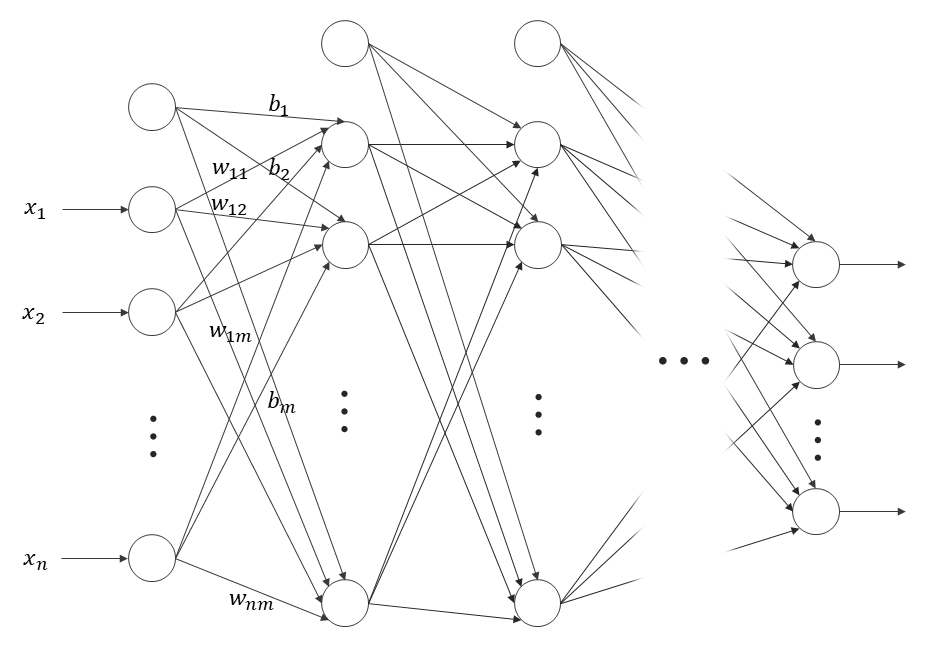
\includegraphics[keepaspectratio, width=120mm]{img/nn.png}
	\caption{ニューラルネットワークのモデルアーキテクチャ}
	\label{fig_nn}
\end{figure}

\begin{align}
  \bm{h}_{\bm{W},~ \bm{b}}(\bm{X}) &= \bm{\phi}(\bm{X}\bm{W} + \bm{b}) \label{nn_layer}
  \\
  \nonumber
  \\
  \bm{X} &= 
  \begin{bmatrix}
    & x_1 & x_2 & \cdots & x_n  &
  \end{bmatrix}
  \label{nn_x}
  \\
  \nonumber
  \\
  \bm{W} &=
  \begin{bmatrix}
    & w_{11} & w_{12} & \cdots & w_{1m} & \\
    & w_{21} & w_{22} & \cdots & w_{2m} & \\
    & \vdots & \vdots & \ddots & \vdots & \\
    & w_{n1} & w_{n2} & \cdots & w_{nm} & \\
  \end{bmatrix}
  \label{nn_w}
  \\
  \nonumber
  \\
  \bm{b} &=
  \begin{bmatrix}
    & b_1 & b_2 & \cdots & b_n  &
  \end{bmatrix}
  \label{nn_b}
\end{align}

$\bm{X}$は数値化したデータの特徴を示す特徴量,
$\bm{W}$はノード間の関係の強さを示す接続重み,
$\bm{b}$は一般に1を要素とするバイアスニューロンと呼ばれるものである.

ニューラルネットワークは脳細胞と似たように,個々のノード間の関係の強さを調節して機能する.
具体的には,式(\ref{nn_update_weight})に示すようにノードの理想の出力$\hat{y}_j$と実際の出力$y_j$の差を利用するなどして次の学習時の接続重みを更新する.

\begin{align}
  w_{i, j}^{(next~ step)} &= w_{i, j} + \eta~ (y_j - \hat{y}_j)~ x_i
  \label{nn_update_weight}
  \\
  \eta &= Const.
  \label{nn_learning_rate}
\end{align}

種々のタスクに特化した機械学習モデルは,このニューラルネットワークの各ノードの接続方法や追加の関数を工夫して作成される.

\subsection{損失関数}
損失関数は,機械学習モデルの出力層の出力と正解の出力との誤差を表す関数であり,モデルの学習ごとの性能指標として用いられる\cite{aurellen20}.
本研究のクラス分類では,2クラスの分類によく用いられる損失関数として
% 式\ref{mse}に示す平均二乗誤差
式(\ref{log_loss})に示すLog Loss
を用いた.

% \begin{align}
%   MSE\left(\bm{X}^{\left( i \right)}, h \right)
%   &= \frac{1}{m} \sum_{i=1}^m 
%   \left\{
%     h \left( \bm{X}^{\left( i \right)} \right)
%     -
%     \hat{y}^{\left( i \right)}
%   \right\}^2
%   \label{mse}
% \end{align}

% $h \left( \bm{X}^{\left( i \right)} \right)$
% はモデルの出力,
% $\hat{y}^{\left( i \right)}$
% は正解の出力を表し,
% m個のデータについてこれらの差の二乗の平均を求めて誤差としている.

\begin{align}
  J(\theta)&=-\frac{1}{m} \sum_{i=1}^{m}\left[y^{(i)} \log \left(\hat{p}^{(i)}\right)+\left(1-y^{(i)}\right) \log \left(1-\hat{p}^{(i)}\right)\right]
  \label{log_loss}
  \\
  % \hat{y}&=\left\{
  % \begin{array}{ll}
  %   0 & \text { if } \hat{p}<0.5 \\
  %   1 & \text { if } \hat{p} \geqq 0.5
  % \end{array}\right.
  % \label{logistic_predict}
  y^{(i)}&=\left\{
    \begin{array}{l}
      0 \\
      1 
    \end{array}
  \right.
  \label{logistic_predict}
  \\
  \hat{p}
  &=\left[ \hat{p}^{(1)}~ \hat{p}^{(2)}~ \cdots~ \hat{p}^{(m)} \right]
  =h_{\theta}(\mathbf{x})
  =\sigma\left(\mathbf{x}^{\top} \theta\right)
  \label{logistic_probability}
  \\
  \sigma(t)&=\frac{1}{1+\exp (-t)}
  \label{sigmoid}
\end{align}

$y^{(i)}$は入力する特徴$\mathbf{x}$の個々の要素のラベルで,$\hat{p}$は$\mathbf{x}$の個々の要素についてモデルが予測したラベルが1となる確率である.
Log Loss$J(\theta)$は個々の$y^{(i)}$と$\hat{p}^{(i)}$の差が大きいほど大きくなり,この差が小さいほど0に漸近する.
式(\ref{logistic_probability})の$\theta$は特徴$\mathbf{x}$のどの要素を重視するかを設定する重み係数である.
式(\ref{sigmoid})の$\sigma(t)$はシグモイド関数と呼ばれる連続関数であり,実数tを入力したとき図\ref{fig_sigmoid}のように確率の範囲$(0, 1)$で実数を出力する.シグモイド関数を用いることで,$(0, 1)$の範囲にないモデルの出力を$(0, 1)$の範囲に落とし込むことができる.

% $h \left( \bm{X}^{\left( i \right)} \right)$
% はモデルの出力,
% $\hat{y}^{\left( i \right)}$
% は正解の出力を表し,
% m個のデータについてこれらの差の二乗の平均を求めて誤差としている.
ニューラルネットワークの重みの更新は損失関数を基に行われ,勾配降下法や誤差逆伝播法を用いて効率よく計算される.
% シグモイド関数は微分をしやすく,勾配降下法や誤差逆伝播法に用いやすい.

\begin{figure}[H]
  \centering
  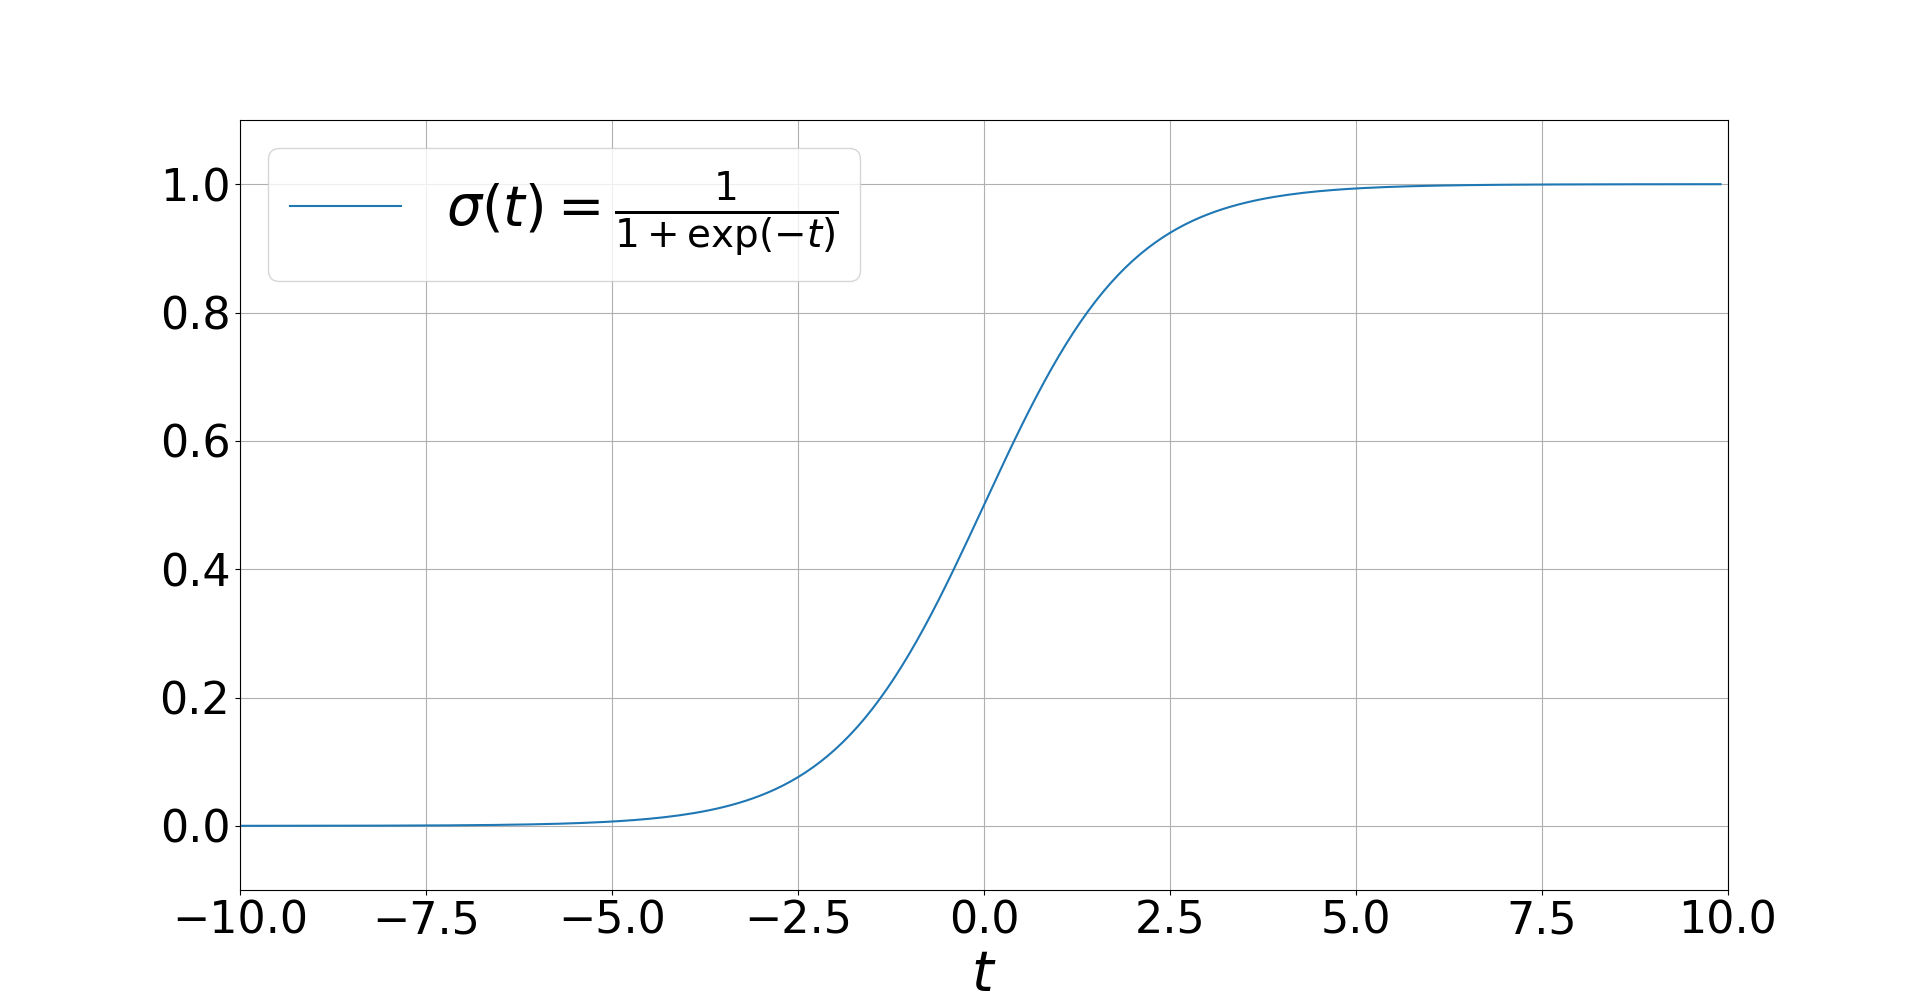
\includegraphics[keepaspectratio, width=120mm]{img/sigmoid.png}
  \caption{シグモイド関数}
  \label{fig_sigmoid}
\end{figure}

% @see p.41, 115

% \subsection{勾配降下法}
% 勾配降下法は,

% @see 4.2 p.~~90~~, 119-139, 174
% 勾配降下法も最適化の話なので省略可能
% 誤差逆伝播法は勾配降下法の効率化なので省略可能 290-294

%%%%%%%%%%%%%%%%%%%%%%%%%%%%%%

\section{機械学習の文章データへの応用}
\label{apply_for_time_series_data}
日々の気温や株価,Webサイトのアクセス数のように,時刻ごとに計測されるデータを時系列データという\cite{aurellen20}.
上記の例では,過去のデータの傾向から未来のデータを予測することができる.
特に,予測したい時刻$t$のデータの直前のデータは,時刻$t$のデータに類似していたり時刻$t$周辺のデータの変化率の情報を含んでいたりするため,予測に大きく役立つ.

時刻を文章内の単語の順番に対応させると,文章データも時系列データと見なすことができる.
文章内の任意の単語は,その前後の単語の意味や文法の傾向から予測することができる.
特に,予測したい単語の直前・直後の単語は,単語の予測の大きなヒントとなる.

本節\ref{apply_for_time_series_data}では,文章をはじめとした時系列データを分析するための機械学習の応用例について記す.
% @see 

\subsection{単語埋め込み}
データのカテゴリを表現する訓練可能な密なベクトルを埋め込みという\cite{aurellen20}.
中でも,単語を表現しようとする埋め込みは単語埋め込みと呼ばれる.

デフォルトでは,ベクトルは無作為な数値で初期化される.
例えば,"NEAR BAY"というカテゴリは,初期状態で$[0.131, 0.890]$といった無作為なベクトルで表現される.
ベクトルの次元数は,目的やモデルの構造によって調節する必要がある.
初期化した単語埋め込みは,意味が似た単語の埋め込み同士は距離を小さくするなど,何らかのアルゴリズムで表現を学習していく.
学習した表現が適切であるほど,単語埋め込みを利用した自然言語処理の機械学習タスクはより精度が増す.
% $v(King) - v(Man) + v(Woman) = v(Queen)$といった加算・減算ができるようになる.
% @see p.430

\subsection{テキストの前処理}
単語埋め込みのように,自然言語処理ではテキストをコンピュータが解釈しやすい数値に変換して処理することが多い.
このとき,コンピュータはテキストを文字の羅列としか見ていないため,Appleとappleを別の単語と見なし,違う数値に変換してしまう.
このような単語の表記揺れは,文章中の単語の出現頻度の情報を不正確なものにする.
表記揺れによって増加した出現頻度の少ない単語が学習のノイズとなってしまうこともある.
従って,テキストに何らかの処理をする前に,大文字を小文字に変換するなどの表記揺れを解消する処理を行う必要がある.
URLやメールアドレスといったユニークな文字の羅列は,出現頻度が極めて少ないノイズとなり得るため,事前に除去しておくと良い.

% @see 週次報告書 2021年10月13日
% @see [自然言語処理における前処理の種類とその威力(2017)](https://qiita.com/Hironsan/items/2466fe0f344115aff177)

\subsection{Attention}
Bahdanauらが2014年に提案したAttentionは,時系列データの機械学習を行う際,出力データと関わりが強い入力データに効率よく比重を与えるモジュールである\cite{aurellen20}\cite{bahdanau_neural_2016}.
モデルにAttentionを組み込むことで無駄なデータの学習が減り,モデルが過去に学習した内容を忘却しにくくなる.
これにより,30語以上の長い文章の機械翻訳タスクの精度が大幅に向上する.

図\ref{fig_attention}に機械翻訳モデルに組み込まれたAttention機構を示す.

\begin{figure}[H]
	\centering
	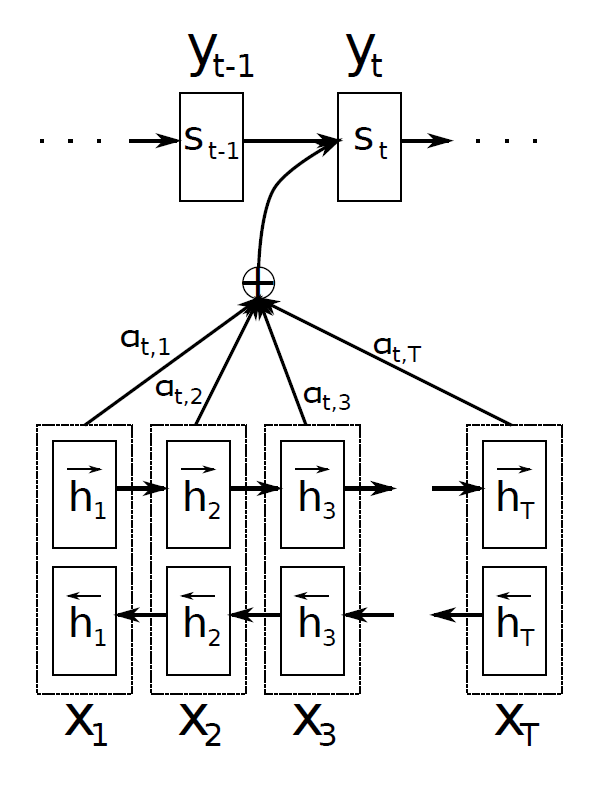
\includegraphics[keepaspectratio, width=120mm]{img/attention.png}
	\caption{入力単語群$(x_1, x_2, ... , x_T)$を基にt番目の出力語$y_t$を生成するAttentionのモデルアーキテクチャ\protect\footnotemark[1]}
	\label{fig_attention}
\end{figure}
\footnotetext[1]{\cite{bahdanau_neural_2016}より引用}

直前に翻訳した単語$y_{t-1}$と過去に翻訳した単語群の情報$s_{t-1}$に,Attentionの式(\ref{attention_c}))を考慮して次の単語$y_t$を予測している.
$\vec{h_i}$は文脈を加味した単語の意味情報をもつベクトルであり,BiGRUと呼ばれるニューラルネットワークを用いて生成されている.

\begin{align}
  c_{i} &= \sum_{j=1}^{T_{x}} \alpha_{i j} h_{j} &
  \label{attention_c}
  \\
  \alpha_{i j} &= \operatorname*{softmax}_j(e_{ij}) = \frac{\exp \left(e_{i j}\right)}{\sum_{k=1}^{T_{x}} \exp \left(e_{i k}\right)}
  \label{attention_alpha}
  \\
  e_{i j} &= a\left(s_{i-1}, h_{j}\right) = v_{a}^{\top} \tanh \left(W_{a} s_{i-1}+U_{a} h_{j}\right)
  \label{attention_e}
\end{align}

式(\ref{attention_alpha})はソフトマックス関数と呼ばれる関数に式(\ref{attention_e})を代入したものであり$\sum_j \alpha_{ij} = 1$となる意味ベクトル$h_j$の重み係数を表す.
式(\ref{attention_e})は,過去に翻訳した単語群の情報$s_{t-1}$と入力単語の意味ベクトル$h_j$を基に,どの単語に比重を置くかを決定するニューラルネットワークである.
式(\ref{attention_e})の$v_{a}^{\top},~ W_{a},~ U_{a}$はニューラルネットワークの重みである.

\subsection{Transformer}
Vaswaniらが2017年に提案したTransformerは,Attentionを組み込んだ翻訳タスクに用いられる機械学習モデルで,2017年の最先端のモデルと比べて数分の1のコストで最大級の精度を有する\cite{aurellen20}\cite{vaswani_attention_nodate}.
時系列データを扱う従来の機械学習にはRNN(Recurrent Neural Network)が多く組み込まれていたが,このモデルは単語を逐次的に処理する仕組みになっており,並列演算が難しい.
一方でTransformerは,RNNを組み込まずに並列演算が可能なAttentionを多く組み込んで時系列データを処理するため,処理コストが低い.

Transformerは,文章を文意を表すベクトルに変換するエンコーダ部分と,そのベクトルを用いて目的の文章を生成するデコーダ部分に分かれるエンコーダ・デコーダモデルの一種である.
図\ref{fig_transformer}に示すTransformerのうち,左半分がエンコーダ,右半分がデコーダである.
エンコーダの入力は翻訳前の文章であり,デコーダの入力はエンコーダの出力と翻訳後の文章である.
デコーダの出力は翻訳中の文章の次の単語の予測確率である.
なお,デコーダに入力される翻訳後の文章は,モデルの学習の際には全文が渡され,予測の際には翻訳中の単語群が渡される.

\begin{figure}[H]
	\centering
	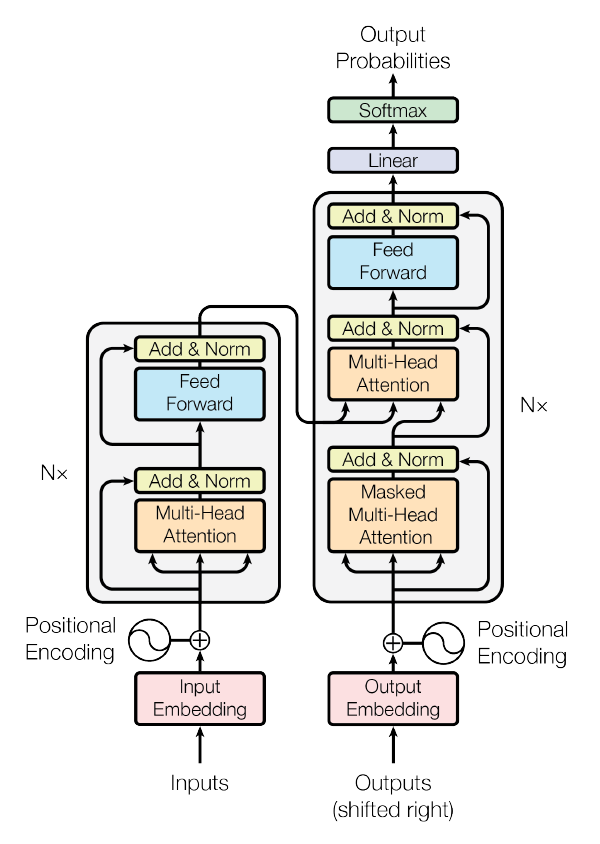
\includegraphics[keepaspectratio, width=120mm]{img/transformer.png}
	\caption{Transformerのモデルアーキテクチャ\protect\footnotemark[2]}
	\label{fig_transformer}
\end{figure}
\footnotetext[2]{\cite{vaswani_attention_nodate}より引用}

Transformerの学習コストを低減する所以となるAttentionは,図\ref{fig_attentions-of-transformer}のように工夫されて組み込まれている.

\begin{figure}[H]
	\centering
	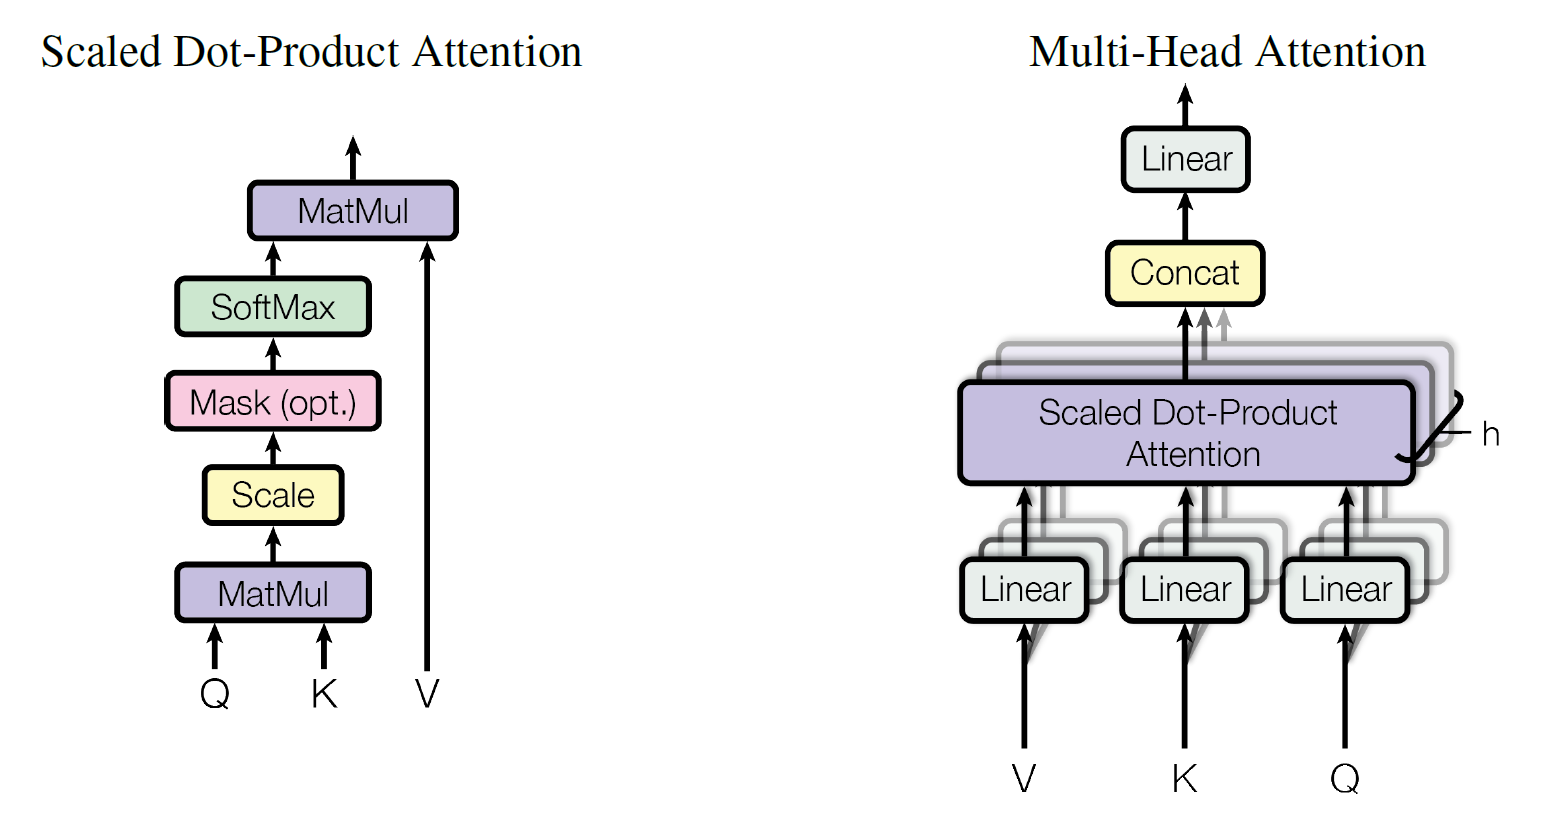
\includegraphics[keepaspectratio, width=120mm]{img/attentions-of-transformer.png}
	\caption{Transformerを構成するMulti-Head Attention(右)とそれを構成すScaled Dot-Product Attention(左)のモデルアーキテクチャ\protect\footnotemark[3]}
	\label{fig_attentions-of-transformer}
\end{figure}
\footnotetext[3]{\cite{vaswani_attention_nodate}より引用}

Scaled Dot-Product Attentionは式(\ref{scaled_dot_product_attention})で表される.
$Q$(Queue)は入力を意味し,式(\ref{scaled_dot_product_attention})は$Q$と$K$(Key)との類似度を基にした重みづけによって出力$V$(Value)を調節するような効果をもつ.

Multi-Head Attentionは式(\ref{multi_head_attention})で表される.
式(\ref{multi_head_attention})を構成する式\ref{scaled_dot_product_attention})の$Q,~ K,~ V$は同値であり,Transformerのデコーダへの入力文をOutput EmbeddingとPositional Encodingで加工したもの(Xとする)を表す.
これらの$Q,~ K,~ V$に$W_i^Q,~ W_i^K,~ W_i^V$を作用させて役割を変えている.
$QW_i^Q$はXのどの部分を処理するかを表し,$KW_i^K$はXの注目の仕方を表し,$VW_i^V$は出力の様子を調整する役割を担う.

\begin{align}
  \text { Attention }(Q, K, V) &= \operatorname{softmax}\left(\frac{Q K^{T}}{\sqrt{d_{k}}}\right) V
  \label{scaled_dot_product_attention}
  \\
  \text { MultiHead }(Q, K, V) &=\text { Concat }\left(\text { head }_{1}, \ldots, \text { head }_{\mathrm{h}}\right) W^{O}
  \label{multi_head_attention}
  \\
  \text { head }_{\mathrm{i}} &=\operatorname{Attention}\left(Q W_{i}^{Q}, K W_{i}^{K}, V W_{i}^{V}\right)
  \label{substituted_scaled_dot_product_attention}
\end{align}

% (教師なし分類にも触れる)
% @see p.549-

\subsection{BERT}
Liuらが2019年に提案したBERT(Bidirectional Encoder Representations from Transformers)は,文の意味や文脈を加味した自然言語処理を行うための機械学習モデルである\cite{aurellen20}\cite{devlin_bert_2019}.
研究者が大規模な計算資源を用いて自然言語の特徴を学習したBERTモデルを公開しており,学習されたモデルに用途に合わせた追加の学習を行うことで,小規模な計算資源で様々な自然言語タスクを高精度で行うことができる.
このような前段階での学習を事前学習,その後の用途に合わせた学習を転移学習と呼ぶ.

図\ref{fig_bert}に中間層が1つのBERTのモデルアーキテクチャを示す.
入力と出力はともに次元が等しいベクトルである.
中間層と出力層にはTransformerのエンコーダ部分が用いており,文から単語の意味を効果的に学習することができる.
また,個々のTransformerエンコーダが前の層の全てのノードから値を受け取っており,文を前から後ろに読む文脈情報と後ろから前に読む文脈情報の両方を加味した学習が可能である.
BERTモデルは,中間層の数や個々のTransformerの数,Transformer内のAttentionの数などを調整し,種々の自然言語処理タスクの性能を上げている.

\begin{figure}[H]
  \centering
  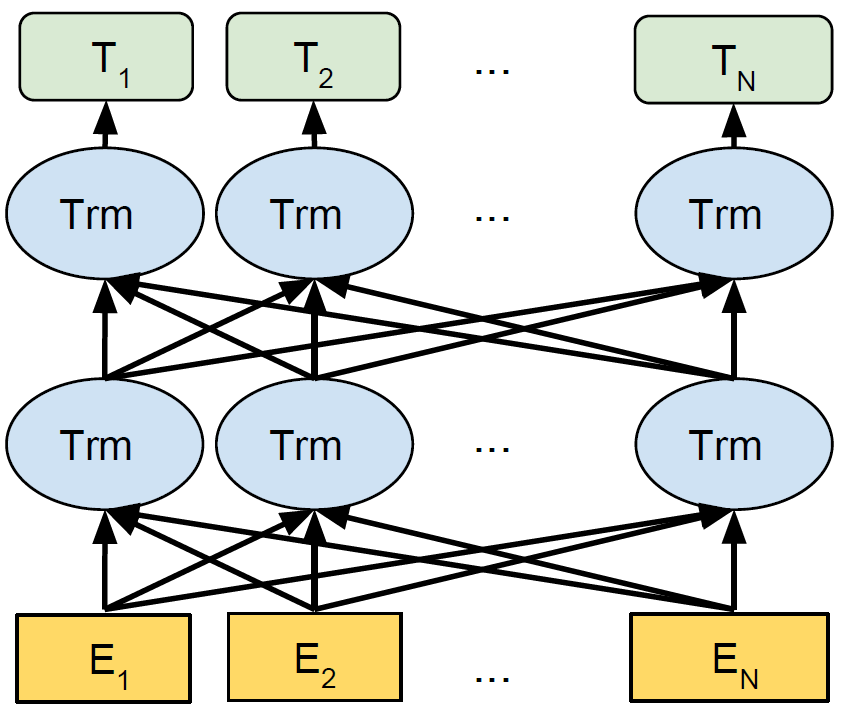
\includegraphics[keepaspectratio, width=120mm]{img/bert.png}
  \caption{中間層が1つのBERTのモデルアーキテクチャ\protect\footnotemark[4]}
  \label{fig_bert}
\end{figure}
\footnotetext[4]{\cite{devlin_bert_2019}の図より一部抜粋}

図\ref{fig_fine_tuning_of_bert}にBERTの事前学習と転移学習の手順を示す.
事前学習で入力するベクトルの要素は,分類のための出力の次元調整に用いる定ベクトル[CLS],入力する2文の単語埋め込み,2文の分割位置を示す定ベクトル[SEP]で構成される.
図中の左の事前学習では,文法や単語の意味の意味を理解するためのMLM(Masked Language Model)としての学習と,文意と文脈を理解するためのNSP(Next Sentence Prediction)としての学習を同時に行う.

MLMとしての学習では,まずモデルに入力する2文の単語の15\%のうち,80\%を文字列[MASK]に置き換え,10\%を無作為に抽出した単語に置き換える.残りの10\%は何も置き換えない.
この置き換えにより,事前学習でしか入力しない文字列[MASK]について,事前学習と転移学習とのミスマッチを低減することができる.
その後,出力されたベクトルの入力でマスクされた位置と同じ位置の要素を使用し,マスク前の単語がどの単語であったかを予測する単語ごとの確率を計算して出力する.
% 1層の全結合層とソフトマックス関数
出力した確率とマスクした正解の単語を基に損失関数を計算し,モデルの重みの更新を行う.

NSPとしての学習では,入力文の50\%を文章中で連続する2文,残りの50\%を文章中で連続しない無作為に抽出された2文として入力する.
入力する2文には,文章中で連続した2文であるかそうでないかのラベル付けがなされている.
その後,出力されたベクトルの[CLS]と同じ位置の要素Cとラベルを使用してどちらの2文であったかの損失関数を計算し,モデルの重みを更新する.

\begin{figure}[H]
	\centering
	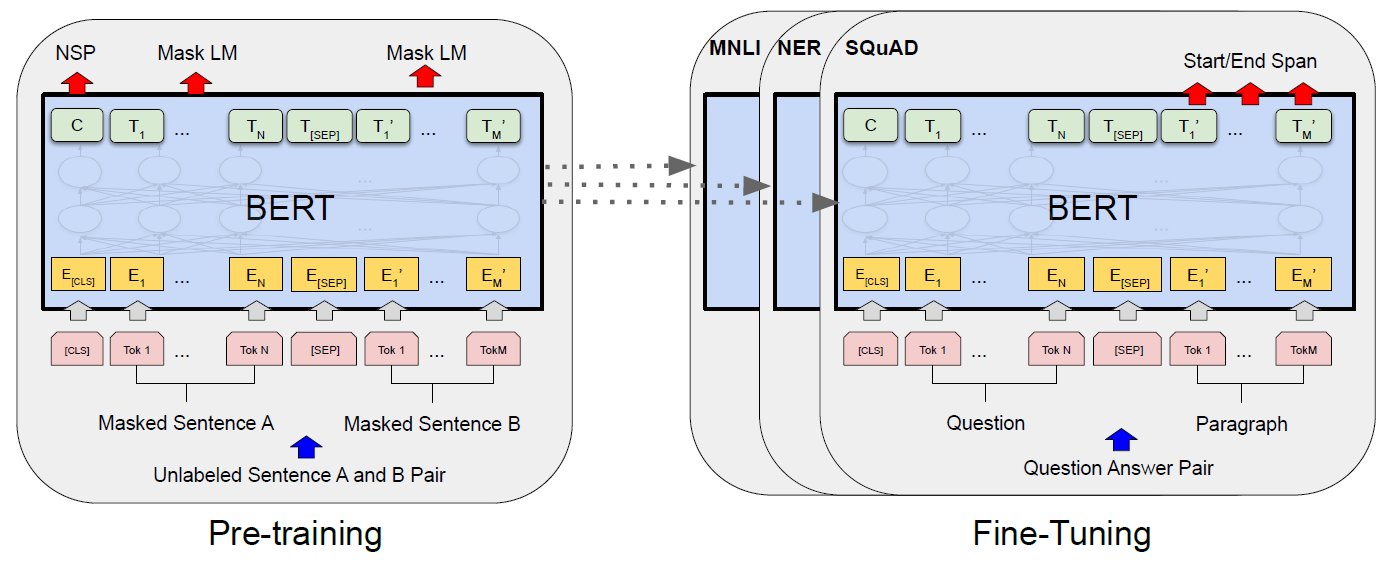
\includegraphics[keepaspectratio, width=120mm]{img/fine-tuning-of-bert.png}
	\caption{BERTの事前学習と転移学習の手順\protect\footnotemark[5]}
	\label{fig_fine_tuning_of_bert}
\end{figure}
\footnotetext[5]{\cite{devlin_bert_2019}より引用}

事前学習の後は,MNLI(Multi-Genre Natural Language Inference),NER(Named Entity Recognition),SQuAD(The Stanford Question Answering Dataset)などの行いたい自然言語処理タスクに合わせて入力と使用する出力の要素を変える.
図\ref{fig_single_sentence_classification_of_bert}に1文のクラス分類のためのBERTの転移学習のモデルアーキテクチャを示す.
この学習では文字列[CLS]と分類したい1文を入力し,[CLS]に対応する出力$\bm{C}$と正解のラベルを基に損失関数の計算を行っている.

% 交差エントロピー
% https://github.com/ThilinaRajapakse/simpletransformers/blob/master/docs/_docs/05-classification-models.md
% 実質ロジスティック回帰 p.150
% class RobertaClassificationHead(nn.Module):
%     """Head for sentence-level classification tasks."""
%     def __init__(self, config):
%         super().__init__()
%         self.dense = nn.Linear(config.hidden_size, config.hidden_size)
%         self.dropout = nn.Dropout(config.hidden_dropout_prob)
%         self.out_proj = nn.Linear(config.hidden_size, config.num_labels)

\begin{figure}[H]
	\centering
	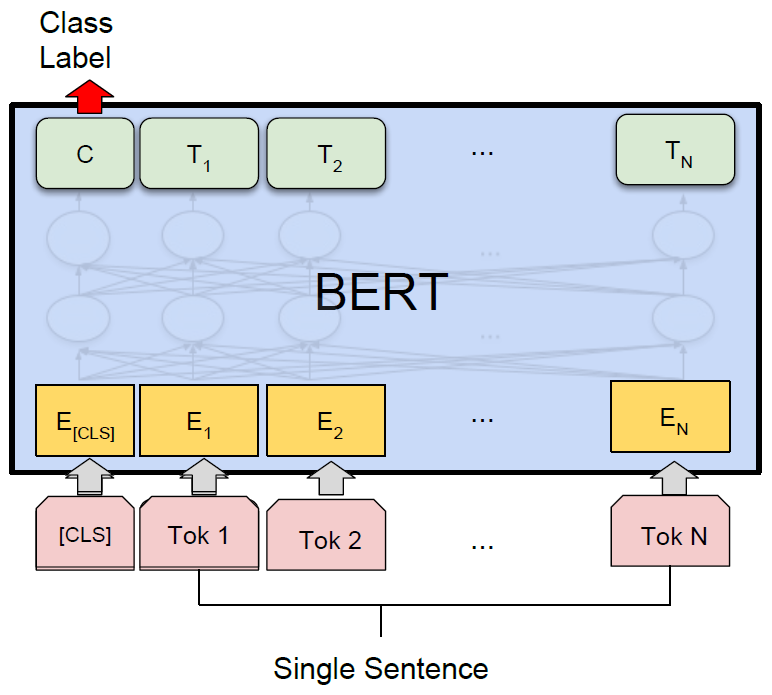
\includegraphics[keepaspectratio, width=120mm]{img/single-sentence-classification-of-bert.png}
	\caption{1文のクラス分類のためのBERTの転移学習\protect\footnotemark[6]}
	\label{fig_single_sentence_classification_of_bert}
\end{figure}
\footnotetext[6]{\cite{devlin_bert_2019}より引用}


% 転移学習 325 345-348 475-477

% @see https://www.youtube.com/watch?v=IaTCGRL41_k&list=PLhDAH9aTfnxL4XdCRjUCC0_flR00A6tJR&index=17
% @see https://data-analytics.fun/2020/05/02/understanding-bert/
% @see https://qiita.com/omiita/items/72998858efc19a368e50

\subsection{RoBERTa}
Devlinらが2019年に提案したRoBERTaはBERTの学習方法を改善した機械学習モデルで,多くの自然言語処理タスクのベンチマークでBERTのスコアを上回る.
RoBERTaのモデルアーキテクチャは図\ref{fig_bert}のBERTと同じものを使用する.
MLMとしての学習でBERTでは10回学習するごとに同じマスクを使用していたため,どの学習でも異なるマスクを使用することでSQuAD(Stanford Question Answering Dataset)とSST-2(The Stanford Sentiment Treebank)のスコアを向上させた.
% 余裕があれば表を挿入
BERTが行っていたNSPとしての学習は比較実験により有効でないことが確認され,RoBERTaではこれを行っていない.
比較実験では,BERTが行ったSEGMENT-PAIRのNSPの学習の代わりにSENTENCE-PAIRのNSPの学習,FULL-SENTENCESのNSPをしない学習,DOC-SENTENCESのNSPをしない学習を行い,NSPの学習を行わなくてもSQuAD,SST-2,MNLI-m(The Multi-Genre Natural Language Inference Matched),RACE(Reading Comprehension)のスコアが概ね向上することを確認した.
% 余裕があれば表を挿入
BERTでは学習データとして250万単語のEnglish Wikipediaと80万単語のBooksCorpusで計16GBのデータを用いていたが,RoBERTaではこれに加えて76GBのCC-News,38GBのOpenWebText,31GBのStoriesを学習した.
さらに,1回の学習で用いるデータサイズ(バッチサイズ)を256から8,000に増やすことで,BERTよりもSQuAD,MNLI-m,SST-2のスコアが向上することを確認した.


表\ref{roberta_glue}にBERTとRoBERTaのGLUE(General Language Understanding Evaluation)タスクのベンチマークスコアを示す.
それぞれのベンチマークでは以下のタスクを行っている.

\begin{itemize}
  \item MNLI(The Multi-Genre Natural Language Inference)
  \begin{itemize}
    \item 2つの文が含意,矛盾,中立のどの関係にあるかを判定
  \end{itemize}
  \item QNLI(Question Natural Language Inference)
  \begin{itemize}
    \item 質問文とともに入力した文が質問に対する正しい回答であるかを判定
  \end{itemize}
  \item QQP(Quora Question Pairs)
  \begin{itemize}
    \item 2つの質問文が同じ意味であるかを判定
  \end{itemize}
  \item RTE(Recognizing Textual Entailment)
  \begin{itemize}
    \item 2つの文が含意関係にあるかを判定
  \end{itemize}
  \item SST(The Stanford Sentiment Treebank)
  \begin{itemize}
    \item 映画のレビュー文がポジティブであるかネガティブであるかを判定
  \end{itemize}
  \item MRPC(Microsoft Research Paraphrase Corpus)
  \begin{itemize}
    \item 2つの文が同じ意味であるかを判定
  \end{itemize}
  \item CoLA(The Corpus of Linguistic Acceptability)
  \begin{itemize}
    \item 英文の文法が正しいかを判定
  \end{itemize}
  \item STS(Semantic Textual Similarity Benchmark)
  \begin{itemize}
    \item ニュースの2つの見出し文の類似度を5段階で評価
  \end{itemize}
\end{itemize}
本研究におけるクラス分類ではSTSのスコアが重要であり,このスコアはRoBERTaの学習方法により90.0から92.4に向上している.

\begin{table}[H]
  \caption{
    BERTとRoBERTaのGLUEタスクのベンチマークスコア.
    全ての結果は24層のアーキテクチャを使用し,5回の実行結果の中央値を取っている.
    \protect\footnotemark[7]
    }
  \centering
  \vspace{3.0mm}
  % {\tabcolsep=0.13cm
    % \begin{tabular}{lccccccccc}
    % \hline
    % & \textbf{MNLI} & \textbf{QNLI} & \textbf{QQP} & \textbf{RTE} & \textbf{SST} & \textbf{MRPC} & \textbf{CoLA} & \textbf{STS} & \textbf{WNLI} \\
    % \hline
    % $\text{BERT}_{\text{LARGE}}$ & 86.6 & 92.3 & 91.3 & 70.4 & 93.2 & 88.0 & 60.6 & 90.0 & - \\
    % RoBERTa & \textbf{90.2} & \textbf{94.7} & \textbf{92.2} & \textbf{86.6} & \textbf{96.4} & \textbf{90.9} & \textbf{68.0} & \textbf{92.4} & 91.3 \\
    \begin{tabular}{lcccccccc}
    \hline
    & \textbf{MNLI} & \textbf{QNLI} & \textbf{QQP} & \textbf{RTE} & \textbf{SST} & \textbf{MRPC} & \textbf{CoLA} & \textbf{STS} \\
    \hline
    $\text{BERT}_{\text{LARGE}}$ & 86.6 & 92.3 & 91.3 & 70.4 & 93.2 & 88.0 & 60.6 & 90.0 \\
    RoBERTa & \textbf{90.2} & \textbf{94.7} & \textbf{92.2} & \textbf{86.6} & \textbf{96.4} & \textbf{90.9} & \textbf{68.0} & \textbf{92.4} \\
    \hline
  \end{tabular}
  % }
  \label{roberta_glue}
\end{table}
\footnotetext[7]{\cite{liu_roberta_2019}より一部抜粋}

% @see https://note.com/npaka/n/n5086fc19c5fc

% @see https://data-analytics.fun/2020/05/08/understanding-roberta/
% @see https://github.com/pytorch/fairseq/tree/main/examples/roberta
% @see https://tensorflow.classcat.com/2021/05/16/huggingface-transformers-4-6-pretrained-models/
% @see https://www.youtube.com/watch?v=T7nbrIJtYlE&list=PLhDAH9aTfnxL4XdCRjUCC0_flR00A6tJR&index=22
% @see 

%%%%%%%%%%%%%%%%%%%%%%%%%%%%%%

\section{教師あり学習の評価}
教師あり学習は,訓練データ(教師データ)と呼ばれる特徴を学習したデータとは別に,学習に用いていないテストデータと呼ばれるデータで入出力の評価を行う必要がある\cite{aurellen20}.
この評価は,モデルに未知のデータを入力したときに目的の出力を得るために必要な操作である.

訓練データで目的の出力を得られてもテストデータで目的の出力が得られないとき,モデルは過学習(過剰適合)しているといい,モデルは未知のデータに対応できていない.
過学習は,モデルの学習回数が多く訓練データの特徴を学習しすぎたときや,学習の手法が適切でないときに起こり得る.
一方で,訓練データでも目的の出力を得られていないとき,モデルは過少適合しているという.
過少適合はモデルの学習回数が少なく訓練データの特徴を学習できていないときや,学習の手法が適切でないときに起こり得る.
目的の出力が得られているかどうかは,学習ごとの損失関数の出力の大きさから確認することができる.

同じデータでテストデータの評価を行いたいときは,データを訓練データとテストデータに分割して評価する.
例えば,100件のデータの80件を訓練データとして学習し,学習に用いていない20件のデータをテストデータとして評価を行う.
% 交差検証の可能性を残す

% @see 

\subsection{混同行列を用いた分類器の評価}
分類器の評価では,混同行列を用いたいくつかの評価指標がよく用いられる\cite{aurellen20}.
混同行列は,分類器の入力の$n$種類のラベルと出力の$n$種類のラベルの計$n^2$組の組み合わせについて,それぞれの数を要素とした$n$次正方行列である.

表\ref{confusion_matrix}に10件のデータを0か1かの2値ラベルで分類したときの混同行列の例を示す.
評価指標の計算で着目するクラスを陽性クラス(positive class),その他のクラスを陰性クラス(negative class)といい,表\ref{confusion_matrix}では1を陽性クラス,0を陰性クラスとして考える.
表\ref{confusion_matrix}の2件のデータは正しく分類した陰性クラスであり,真陰性(TN; true negative)があるという.
表\ref{confusion_matrix}の1件のデータは誤って陽性クラスだと分類した陰性クラスであり,偽陽性(FP; false positive)があるという.
表\ref{confusion_matrix}の3件のデータは誤って陰性クラスだと分類した陽性クラスであり,偽陰性(FN; false negative)があるという.
表\ref{confusion_matrix}の4件のデータは正しく分類した陽性クラスであり,真陽性(TP; true positive)があるという.
以降の小小節
\ref{subsubsection_precision},
\ref{subsubsection_recall},
\ref{subsubsection_mcc},
では,これらTN,FN,FP,TPを用いて計算した評価指標である適合率,再現率,マシューズ相関係数について記す.

\begin{table}[H]
  \caption{
    混同行列の例
    }
  \vspace{3mm}
  \centering
    \begin{tabular}{c|cc}
     & 予測は0 & 予測は1 \\
    \hline
    入力は0 & 2 & 1 \\
    入力は1 & 3 & 4
  \end{tabular}
  % }
  \label{confusion_matrix}
\end{table}

% @see 92-94 104-106
% @see https://zellij.hatenablog.com/entry/20120214/p1
% @see https://www.datarobot.com/jp/blog/matthews-correlation-coefficient/


\subsubsection{適合率}
\label{subsubsection_precision}
適合率(precision)は,陽性クラスだと分類したデータのうち真陽性クラスであるデータの割合である\cite{aurellen20}.
表\ref{confusion_matrix}の例では,ラベルが1だと予測データのうち実際に1であったデータの割合を指す.
したがって,式(\ref{precision})のように適合率が計算される.

\begin{align}
  precision ~=~ \frac{TP}{TP+FP} ~=~ \frac{4}{4+1} ~=~ 0.8
  \label{precision}
\end{align}

適合率は,数ある映像から子どもに観せても安心な映像を検出する分類器などで重視される.
観せて安心な映像を陽性クラスの映像だとしたとき,分類器の適合率が高ければ,観せて安心な映像だと分類した映像の多くは真に観せて安心な映像であることが多い.


\subsubsection{再現率}
\label{subsubsection_recall}
再現率(recall)は,陽性クラスのデータのうち真陽性クラスであるデータの割合である\cite{aurellen20}.
表\ref{confusion_matrix}の例では,ラベルが1のデータのうち予測も1であったデータの割合を指す.
したがって,式(\ref{recall})のように再現率が計算される.

\begin{align}
  recall ~=~ \frac{TP}{TP+FN} ~=~ \frac{4}{4+3} ~\sim~ 0.57
  \label{recall}
\end{align}

再現率は,監視カメラに映る人物の映像から万引き犯の映像を検出する分類器などで重視される.
万引き犯の映像を陽性クラスの映像だとしたとき,分類器の再現率が高ければ,万引き犯の映像の多くは予測も万引き犯の映像となる.

適合率と再現率は一般にトレードオフの関係にあり,分類器の目的によってそれぞれの評価指標をどれほど重要視するかを考慮する必要がある.
上述の監視カメラの例では,適合率が低く万引き犯だと分類した映像のいくつかが万引き反でない人物となってしまうことよりも,再現率が高く確実に万引き犯を検出できることの方が重要である.


\subsubsection{マシューズ相関係数}
\label{subsubsection_mcc}
Matthewsが1975年に提案したマシューズ相関係数(MCC;Matthews Correlation Coefficient)は,混同行列を基に分類器の精度を総合的に評価する指標で,TP,TN,FP,FNの数が不均衡なときにも頑健に評価できる\cite{chicco_advantages_2020}.
マシューズ相関係数は式(\ref{mcc})のように計算される$[-1, 1]$の範囲の実数値であり,この値が大きいほど分類器の精度が高いといえる.
\begin{align}
  MCC ~=~ \frac{\mathrm{TP} \times \mathrm{TN}-\mathrm{FP} \times \mathrm{FN}}{\sqrt{(\mathrm{TP}+\mathrm{FP}) \times(\mathrm{TP}+\mathrm{FN}) \times(\mathrm{TN}+\mathrm{FP}) \times(\mathrm{TN}+\mathrm{FN})}}
  \label{mcc}
\end{align}

% (1*1-0*0)/(1*1*1*1)^-1 = 1
% (0*0-1*1)/(1*1*1*1)^-1 = -1
% @see https://www.datarobot.com/jp/blog/matthews-correlation-coefficient/

\section{文章の距離の算出}
\label{section_sentence_distance}
後述のクラスタリングを行うにあたり,クラスタリングに必要な文章の距離(非類似度)の算出法について記す.
本節\ref{section_sentence_distance}では,小節\ref{subsection_sentence_bert}で文章を埋め込みに変換するSentence-BERTについて説明し,小節\ref{subsection_cosine_distance}で変換した埋め込みを用いて計算するコサイン距離について説明する.

\subsection{Sentence-BERT}
\label{subsection_sentence_bert}
Reimersらが2019年に提案したSentence-BERTは,文章の埋め込みを生成するためのBERTを転移学習した機械学習モデルである\cite{reimers_sentence-bert_2019}.
図\ref{fig_sentence_bert}にSentence-BERTのモデルアーキテクチャを示す.
Sentence-BERTでは転移学習済みのBERTに1つの文を入力し,出力したベクトル群にpoolingと呼ばれる情報の抽出処理を行って文章の埋め込みを得る.
転移学習では,埋め込みを応用したSTSタスクなどの精度を上げるために,
% 3つ関数Classification Objective Function,Regressioon Objective Function,Triplet Objective Functionを用いた
3種類の工夫された学習が行われている.
poolingでは3つの手法が比較されており,BERTで出力したベクトル群の平均を埋め込みとする手法が最もSTSタスクのスコアが優れていた.

% @see 3. Model


\begin{figure}[H]
	\centering
	% 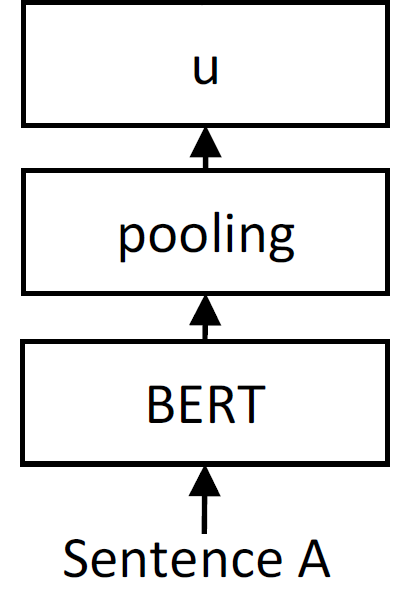
\includegraphics[keepaspectratio, width=120mm]{img/sentence-bert.png}
	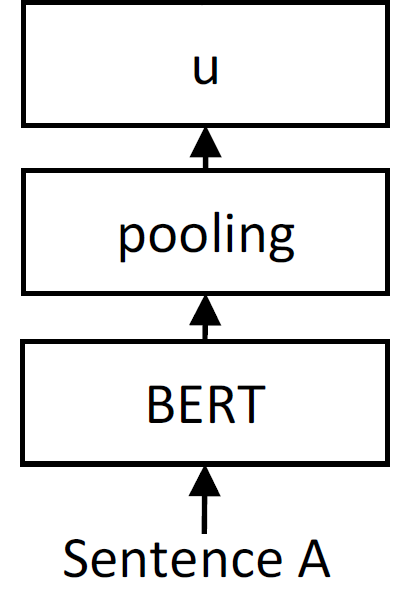
\includegraphics[keepaspectratio, width=60mm]{img/sentence-bert.png}
	\caption{Sentence-BERTのモデルアーキテクチャ\protect\footnotemark[8]}
	\label{fig_sentence_bert}
\end{figure}
\footnotetext[8]{\cite{reimers_sentence-bert_2019}の図より一部抜粋}

BERTやRoBERTaで1万文から最も意味的類似度が高い2文を得たいとき,図\ref{fig_fine_tuning_of_bert}のように2文同時に入力すると$\frac{10000(10000-1)}{2}=49995000$回の実行が必要であり,Reimersらの実験では65時間の処理を要した.
そこでReimersらは,BERTやRoBERTaに1文を入力して単語埋め込みを得る処理を$10000$回行い,埋め込み間の類似度を計算し,処理時間を約5秒に短縮した.
埋め込み間の類似度には,式(\ref{cosine_similarity})に示すコサイン類似度が用いられている.

\begin{align}
  \text{cos-sim}\left(\bm{u}, \bm{v}\right) = \frac{\bm{u} \cdot \bm{v}}{\|\bm{u}\|\|\bm{v}\|}
  \label{cosine_similarity}
\end{align}

表\ref{sentence_bert_evaluation}にSentEvalツールキットを用いた文埋め込みの比較評価を示す.
表より,Sentence-BERTは多くの自然言語処理タスクにおいて2019年の最先端のスコアを有することがわかる.

\begin{table}[H]
  \caption{
    SentEvalツールキットを用いた文埋め込みの比較評価
    \protect\footnotemark[9]
    }
  \vspace{3mm}
  \centering
  {\tabcolsep=0.1cm
    \begin{tabular}{l|cccccccc}
      \hline Model & MR & CR & SUBJ & MPQA & SST & TREC & MRPC & Avg. \\
      \hline Avg. GloVe embeddings & $77.25$ & $78.30$ & $91.17$ & $87.85$ & $80.18$ & $83.0$ & $72.87$ & $81.52$ \\
      Avg. fast-text embeddings & $77.96$ & $79.23$ & $91.68$ & $87.81$ & $82.15$ & $83.6$ & $74.49$ & $82.42$ \\
      Avg. BERT embeddings & $78.66$ & $86.25$ & $94.37$ & $88.66$ & $84.40$ & $92.8$ & $69.45$ & $84.94$ \\
      BERT CLS-vector & $78.68$ & $84.85$ & $94.21$ & $88.23$ & $84.13$ & $91.4$ & $71.13$ & $84.66$ \\
      InferSent - GloVe & $81.57$ & $86.54$ & $92.50$ & $\mathbf{9 0 . 3 8}$ & $84.18$ & $88.2$ & $75.77$ & $85.59$ \\
      Universal Sentence Encoder & $80.09$ & $85.19$ & $93.98$ & $86.70$ & $86.38$ & $\mathbf{9 3 . 2}$ & $70.14$ & $85.10$ \\
      \hline SBERT-NLI-base & $83.64$ & $89.43$ & $94.39$ & $89.86$ & $88.96$ & $89.6$ & $\mathbf{7 6 . 0 0}$ & $87.41$ \\
      SBERT-NLI-large & $\mathbf{8 4 . 8 8}$ & $\mathbf{9 0 . 0 7}$ & $\mathbf{9 4 . 5 2}$ & $90.33$ & $\mathbf{9 0 . 6 6}$ & $87.4$ & $75.94$ & $\mathbf{8 7 . 6 9}$ \\
      \hline
    \end{tabular}
  }  
  \label{sentence_bert_evaluation}
\end{table}
\footnotetext[9]{\cite{reimers_sentence-bert_2019}より引用}

% 文章間の意味的類似度の算出を約5秒に短縮し,STSタスクで2019年の最先端のスコアを有している.
% SentenceTransformer(
%   (0): Transformer({'max_seq_length': 128, 'do_lower_case': False}) with Transformer model: BertModel 
%   (1): Pooling({'word_embedding_dimension': 384, 'pooling_mode_cls_token': False, 'pooling_mode_mean_tokens': True, 'pooling_mode_max_tokens': False, 'pooling_mode_mean_sqrt_len_tokens': False})
% )
% @see https://data-analytics.fun/2020/08/04/understanding-sentence-bert/
% @see https://www.vareal.co.jp/column/sentence-bert%E8%AB%96%E6%96%87-%E5%92%8C%E8%A8%B3/
% @see https://github.com/UKPLab/sentence-transformers
% @see https://www.google.com/search?client=firefox-b-d&q=paraphrase-MiniLM-L6-v2


\subsection{コサイン距離}
\label{subsection_cosine_distance}

コサイン距離は,2つのベクトルの角度がどの程度離れているかを表す距離(非類似度)であり,式(\ref{cosine_distance})のように計算される.
コサイン距離は,単語埋め込みや文章の埋め込みの距離の算出によく用いられる.

\begin{align}
  \text{cos-dist}\left(\bm{u}, \bm{v}\right) ~&=~
  1 -
  \text{cos-sim}\left(\bm{u}, \bm{v}\right) ~=~
  1 - \frac{\bm{u} \cdot \bm{v}}{\|\bm{u}\|\|\bm{v}\|}
  \label{cosine_distance}
\end{align}

%%%%%%%%%%%%%%%%%%%%%%%%%%%%%%
\section{階層的クラスタリング}
\label{section_clustering}
クラスタリングは,データの集合を何らかのアルゴリズムに基づいてクラスタと呼ばれる部分集合に分割する教師なし学習である
% \cite{aurellen20}
.
類似したデータをクラスタにまとめることで,データの要約や傾向の分析を行うことができる.

本節\ref{section_clustering}では,小節\ref{subsection_wards_method}でクラスタ間の距離を算出するWard法について説明し,小節\ref{subsection_hierarchical_clustering}でクラスタリングの一種である階層的クラスタリングについて説明する.
% し,小節\ref{subsection_dendrogram}で階層的クラスタリングの工程を可視化するデンドログラムについて説明する.

% @see 木村先生のデータ解析法
% @see 神嶌先生の講義資料

% \subsection{非階層クラスタリング}
% ~
% @see p.12

\subsection{Ward法}
\label{subsection_wards_method}
階層的クラスタリングの処理には,データの部分集合であるクラスタ同士の距離(クラスタ間距離)が必要となる.
クラスタ間距離の算出には単一連結法や最遠隣法など様々な手法が用いられているが,本研究では1963年にWardが提案したWard法(最小分散法)を使用する\cite{murtagh_wards_2014}.
Ward法は異常なデータの値(外れ値)の影響を受けにくく,クラスタ間距離の算出法として広く用いられている.

Ward法では式(\ref{wards_method})に示すように,
併合後のクラスタ$C_{k} \cup C_{c}$の分散と
併合前のクラスタ$C_{k}, C_{c}$のそれぞれの分散の和との差$d_{k c}$をクラスタ間距離とする.

% 分散の実装方法にはユークリッド距離の観点から実装したものと平方ユークリッド距離の観点から実装したものがあるが,本研究ではデンドログラムでの分析で有用なユークリッド距離の観点から実装したものを用いる.
% ユークリッド距離を使うか平方ユークリッド距離を使うかの実装の差がある

\begin{align}
  d_{k c} &= \operatorname{Var} \left( C_{k} \cup C_{c} \right)
  -
  \left(
    \operatorname{Var}\left(C_{k}\right)
    +
    \operatorname{Var}\left(C_{c}\right)
  \right)
  \label{wards_method}
\end{align}

% @see https://docs.scipy.org/doc/scipy/reference/generated/scipy.cluster.hierarchy.linkage.html


\subsection{階層的クラスタリング}
\label{subsection_hierarchical_clustering}
階層的クラスタリング(凝集型クラスタリング)は,図\ref{fig_clustering_example}に示すようにクラスタ間距離が最も近い2つのクラスタを順次1つのクラスタに結合していく手法である.

結合前のクラスタは結合後のクラスタの部分集合となり,最終的には1つのクラスタとなる.
従って階層的クラスタリングは,このような部分集合の階層構造をもつデータの分析に有用である.
どのクラスタ間距離でクラスタの結合を止めるかによって,様々な粒度のクラスタ群を得ることができる.

\begin{figure}[H]
	\centering
	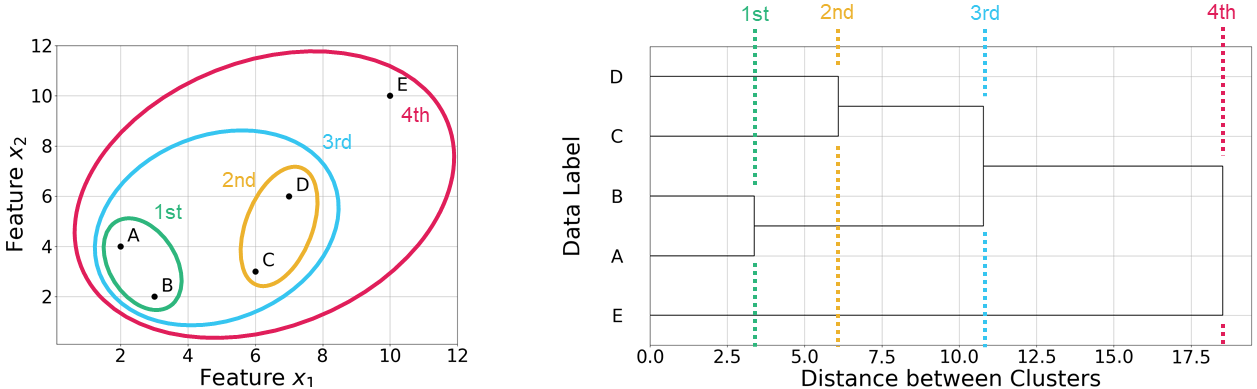
\includegraphics[keepaspectratio, width=120mm]{img/clustering_example.png}
	\caption{階層的クラスタリング}
	\label{fig_clustering_example}
\end{figure}

% @see p.261

% \subsection{デンドログラム}
% \label{subsection_dendrogram}


% \subsection{(その他使用した手法)}
% ~
% % @see 

% \subsection{t-SNE (使うかも)}
% ~
% % @see 

\section{k-NN分類法}
k-NN分類法(k近傍法)は,クラスが既知のデータ群が存在するときに新規に入力したデータのクラスを推定するためのクラス分類手法である\cite{aurellen20}.
新規のデータが入力されたとき,そのデータとの距離が最も近い既存のデータを順にk個選択し,k個のデータのクラスのうち最も多かったクラスを新規のデータのクラスと推定する.
kは事前に設定しておく必要がある.
% 距離の定義
% 教師あり学習

% % @see p.11,24

%%%%%%%%%%%%%%%%%%%%%%%%%%%%%%%%%%%%%%%%%%%%%%%%%%%%%%%%%%%%
\chapter{関連研究}
%%%%%%%%%%%%%%%%%%%%%%%%%%%%%%%%%%%%%%%%%%%%%%%%%%%%%%%%%%%%


%%%%%%%%%%%%%%%%%%%%%%%%%%%%%%
\section{ニュース推薦システムのバイアスの解決}
~
% @see 
% [[1]E. BozdagとJ. van den Hoven, 「Breaking the filter bubble: democracy and design」, Ethics Inf Technol, vol. 17, no. 4, pp. 249–265, 12月 2015, doi: 10.1007/s10676-015-9380-y.](https://link.springer.com/article/10.1007/s10676-015-9380-y?source=post_page-----2afbf9cd8367----------------------)
% - フィルターバブルの回避手法
%     - 目標の誤認?
%         - ユーザーに完全なコントロールを付与
%             - バブルの増大も可能に
%                 - (増大せずにコントロールを付与する方法はないか)
%                 - 両方並べて表示すればいいんじゃない
%         - 視点を多様化するよう検索結果を修正
%             - 民主主義の議論に似ている
%             - 完全な民主主義は難しく,本稿では網羅できない

\subsection{Breaking the filter bubble: democracy and design}
~
% @see 

\subsubsection{(UIでバブルの可視化)(結局表示されるものにバイアスがかかる,行動に繋がらない)}
~
% @see 

\subsubsection{(トピックモデル,LSI, LDAの議論)}
~
% @see 

%%%%%%%%%%%%%%%%%%%%%%%%%%%%%%
\section{話題の定量化によるニュース推薦手法}
~
% @see 

\subsection{トピックマップ}
~
% @see 

\subsection{Labeled Bilingual Topic Model for Cross-Lingual Text Classification and Label Recommendation}
~
% @see 

\subsubsection{(LDAの利用)}
~
% @see 

%%%%%%%%%%
% \section{LSI}
~
% @see 

%%%%%%%%%%%%%%%%%%%%%%%%%%%%%%
% \section{(要追加調査:比較評価できる推薦手法)(出来事,主張に着目するシステムなど)}
\section{主張の文のクラスタリングを行う研究}
% ~
% @see 

\subsection{Scalable Fact-checking with Human-in-the-Loop}

Yangらは,ニュース読者が出来事を正確かつ迅速に把握できるように
階層的クラスタリングを用いて記事に対するツイートの主張をグループ化する手法を提案した\cite{yang_scalable_2021}.
この研究ではCOVID-19の話題に限定した主張の文をグループ化しているが,この手法を記事に適用した場合,多くの話題について主張のまとまりが生成されることになる.
これでは,COVID-19の飲み薬やワクチンなど異なる話題に含まれる安全性に関する共通した主張の文がグループ化されるため,読者が興味を持っている出来事の異なる主張の収集に時間を要してしまう.

% TODO
% クラスタリングについて詳しく
% 図を利用
% クラスタ数が低減していないことに言及

% \subsection{Investigating COVID-19 News Across Four Nations A Topic Modeling and Sentiment Analysis Approach}
% ~
% @see 

\subsubsection{トピックモデル,top2vec, roberta}
~
% @see 

%%%%%%%%%%
% \section{tf-idf -->}
~
% @see 
%  <!-- SCDV -->


%%%%%%%%%%%%%%%%%%%%%%%%%%%%%%%%%%%%%%%%%%%%%%%%%%%%%%%%%%%%
\chapter{提案手法}
%%%%%%%%%%%%%%%%%%%%%%%%%%%%%%%%%%%%%%%%%%%%%%%%%%%%%%%%%%%%
\label{chapter_method}

本研究では,記事の文章が出来事を述べる文と主張を述べる文に二分できると仮定する.
図\ref{fig_method_abstract}に提案手法の概要を示す.

\begin{figure}[H]
	\centering
	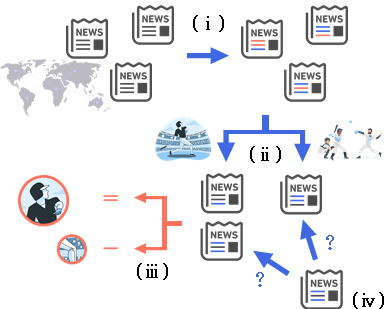
\includegraphics[keepaspectratio, width=120mm]{img/method_abstract.png}
	\caption{
    提案手法の概要
    \newline
    \qquad\quad(\ajroman{1})
    記事の文章を出来事の文と主張の文に分類する
    \newline
    \qquad\quad(\ajroman{2})
    出来事の文章の類似度で記事をクラスタリングする
    \newline
    \qquad\quad(\ajroman{3})
    主張の文の類似度で主張の文をクラスタリングする
    \newline
    \qquad\quad(\ajroman{4})
    読者が興味を持っている記事と同じ出来事を扱う記事のクラスタを
    \newline
    \qquad\qquad\quad
    同定し,そのクラスタに紐づく主張の文をクラスタごとにまとめ,
    \newline
    \qquad\qquad\quad
    記事とともに読者に提示・推薦する
  }
	\label{fig_method_abstract}
\end{figure}

第\ref{chapter_method}章は全4節で構成される.
節\ref{section_term_definition}では本研究で使用する語彙の定義を行い,
節\ref{section_method_detail}では図\ref{fig_method_abstract}に示した提案手法の詳細を説明する.
節\ref{section_select_dataset}では提案手法に必要なデータセットの選定について説明し,
節\ref{section_preprocessing_data}では選定したデータセットの前処理について説明する.

%%%%%%%%%%%%%%%%%%%%%%%%%%%%%%
\section{使用する語彙の定義}
\label{section_term_definition}
~
% @see 

\subsection{文と文章}
~
% @see 

\subsection{出来事の文}
~
% @see 

\subsection{主張の文}
~
% @see 

\subsection{文が示す話題の類似度}
~
% @see 

%%%%%%%%%%%%%%%%%%%%%%%%%%%%%%
\section{記事の出来事と主張のクラスタを用いた多言語ニュース推薦}
\label{section_method_detail}
~
% @see 

% フィルターバブル問題を緩和する策として,推薦アルゴリズムの公開,個人が推薦アルゴリズムを管理できるオプションの作成,UIの工夫によるバブルの可視化がある.一方で,個人が推薦アルゴリズムを微調節したところで完全に情報の泡から脱することはできないとの指摘もある.UIでバブル内外を可視化しきるのは不可能 情報が多い 手軽

% (to 提案手法)特定の地域の似た文化と価値観を持つ者同士に向けて記事を提供し,読者にコメントさせる事は,エコーチェンバー問題による情報の偏りを生むと考える.

\subsection{手法概要}
~
% @see 

\subsection{クラスタリングの順序の検討}
~
% @see 

\subsection{(その他報告会などで議論したこと)}
~
% @see 

%%%%%%%%%%%%%%%%%%%%%%%%%%%%%%
\section{データセットの選定}
\label{section_select_dataset}
~
% @see 

\subsection{出来事の文と主張の文の分類器の学習データ(IBM Debater Datasetの議論)}
~
% @see 

\subsection{分類とクラスタリングを行うデータ(covid-19-articlesの議論)}
~
% @see 

%%%%%%%%%%<!-- 
% \section{Japanese fakenews dataset -->}
~
% @see 

%%%%%%%%%%%%%%%%%%%%%%%%%%%%%%
\section{データの前処理}
\label{section_preprocessing_data}
~
% @see 

\subsection{自然言語処理のためのテキストの前処理(前処理の種類,なぜ前処理するのかなどの議論)}
~
% @see 

\subsection{(その他工夫した前処理)}
~
% @see 


%%%%%%%%%%%%%%%%%%%%%%%%%%%%%%%%%%%%%%%%%%%%%%%%%%%%%%%%%%%%
\chapter{実装}
%%%%%%%%%%%%%%%%%%%%%%%%%%%%%%%%%%%%%%%%%%%%%%%%%%%%%%%%%%%%


%%%%%%%%%%%%%%%%%%%%%%%%%%%%%%
\section{システムの設計指針(入出力,使い方など)}
~
% @see 

%%%%%%%%%%%%%%%%%%%%%%%%%%%%%%
\section{システム構成(モジュールの説明)}
~
% @see 

%%%%%%%%%%%%%%%%%%%%%%%%%%%%%%
\section{実装環境(PCスペック,ライブラリバージョンなど)}
~
% @see 

%%%%%%%%%%%%%%%%%%%%%%%%%%%%%%
\section{データの前処理}
~
% @see 

\subsection{正規表現による前処理(awkの正規表現などの議論)}
~
% @see 

\subsection{省略のピリオドに注意した文章の分割(Stanza, spacyの議論)}
~
% @see 

%%%%%%%%%%%%%%%%%%%%%%%%%%%%%%
\section{出来事の文と主張の文の分類}
~
% @see 

\subsection{Simple Transformers}
~
% @see 

%%%%%%%%%%%%%%%%%%%%%%%%%%%%%%
\section{出来事の文章のクラスタリング}
~
% @see 

\subsection{(要検討)}
~
% @see 

%%%%%%%%%%%%%%%%%%%%%%%%%%%%%%
\section{主張の文のクラスタリング}
~
% @see 

\subsection{(要検討)}
~
% @see 


%%%%%%%%%%%%%%%%%%%%%%%%%%%%%% 
% \section{仮説}
~%% @see 
 評価実験を設計するにあたり以下3件の仮説を立てる.
% \begin{itemize}
%   \item 仮説1) .
%   \item 仮説2) 
%   \item 仮説3) 
% \end{itemize}
% この3件の仮設は,それぞれ以下の考察に基づき設定されている.
% 仮説1は...


%%%%%%%%%%%%%%%%%%%%%%%%%%%%%%%%%%%%%%%%%%%%%%%%%%%%%%%%%%%%
\chapter{実験}
%%%%%%%%%%%%%%%%%%%%%%%%%%%%%%%%%%%%%%%%%%%%%%%%%%%%%%%%%%%%


%%%%%%%%%%%%%%%%%%%%%%%%%%%%%%
\section{出来事の文と主張の文の分類}
~
% @see 

\subsection{実験方法}
~
% @see 

\subsection{実験結果}
~
% @see 

\subsection{実験の考察}
~
% @see 

\subsection{(試行錯誤)}
~
% @see 

%%%%%%%%%%%%%%%%%%%%%%%%%%%%%%
\section{出来事の文章のクラスタリング}
~
% @see 

\subsection{実験方法}
~
% @see 

\subsection{実験結果}
~
% @see 

\subsection{実験の考察}
~
% @see 

\subsection{(試行錯誤)}
~
% @see 

%%%%%%%%%%%%%%%%%%%%%%%%%%%%%%
\section{主張の文のクラスタリング}
~
% @see 

\subsection{実験方法(クラスタの階層の基準ごとの評価)}
~
% @see 

\subsection{実験結果}
~
% @see 

\subsection{実験の考察}
~
% @see 

\subsection{(試行錯誤)}
~
% @see 

%%%%%%%%%%%%%%%%%%%%%%%%%%%%%%
\section{(他の研究との比較実験)}
~
% @see 

\subsection{実験方法}
~
% @see 

\subsection{実験結果}
~
% @see 

\subsection{実験の考察}
~
% @see 

\subsection{(試行錯誤)}
~
% @see 


%%%%%%%%%%%%%%%%%%%%%%%%%%%%%%%%%%%%%%%%%%%%%%%%%%%%%%%%%%%%
\chapter{結果と考察}
%%%%%%%%%%%%%%%%%%%%%%%%%%%%%%%%%%%%%%%%%%%%%%%%%%%%%%%%%%%%


%%%%%%%%%%%%%%%%%%%%%%%%%%%%%%
\section{既存手法との比較}
~
% @see 

%%%%%%%%%%%%%%%%%%%%%%%%%%%%%%
\section{提案手法の妥当性}
~
% @see 

\subsection{入力と出力の妥当性}
~
% @see 

\subsection{処理速度の妥当性(分散システムの議論も)}
~
% @see 

%%%%%%%%%%%%%%%%%%%%%%%%%%%%%%
\section{(結果を基に検討)}
~
% @see 

%%%%%%%%%%%%%%%%%%%%%%%%%%%%%%%%%%%%%%%%%%%%%%%%%%%%%%%%%%%%
\chapter{まとめと展望}
%%%%%%%%%%%%%%%%%%%%%%%%%%%%%%%%%%%%%%%%%%%%%%%%%%%%%%%%%%%%


%%%%%%%%%%%%%%%%%%%%%%%%%%%%%%
\section{まとめ}
~
% @see 

%%%%%%%%%%%%%%%%%%%%%%%%%%%%%%
\section{今後の展望}
~%% @see 
 \section{データセットの相性(ディベートとニュース)}
~
% @see 

%%%%%%%%%%%%%%%%%%%%%%%%%%%%%%%%%%%%%%%%%%%%%%%%%%%%%%%%%%%%
\chapter*{謝辞}
\addcontentsline{toc}{chapter}{謝辞}
%%%%%%%%%%%%%%%%%%%%%%%%%%%%%%%%%%%%%%%%%%%%%%%%%%%%%%%%%%%%

(参考文献は最後に整形します)

%%%%%%%%%%%%%%%%%%%%%%%%%%%%%%%%%%%%%%%%%%%%%%%%%%%%%%%%%%%%
\bibliographystyle{junsrt}
\bibliography{ref.bib}
%%%%%%%%%%%%%%%%%%%%%%%%%%%%%%%%%%%%%%%%%%%%%%%%%%%%%%%%%%%%

\end{document}
